\section{The global view of star formation}
\label{sec:global}

In the following section, we summarise the global view of star formation in the CMZ. 
Due to the highly embedded nature of forming stars, determining star formation rates (SFR) relies on the emission produced either directly from, or indirectly by, star formation over the lifetime of the emission mechanism.
In \S \ref{sec:SFR:current} we review the recent body of literature dedicated to measuring the SFR in the CMZ. As we will see, the SFRs independently derived from various methods, including source counting and integrated light measurements, point to a SFR that has been more or less constant at a value of $\simeq0.07$\,\msunyr \ for at least the last 5\,Myr (Table\,\ref{tab:SFR}).
In \S\ref{subsec:SFR:starformationhistory} and \S\ref{subsec:SFR:timeevolution} we consider the star formation history of the CMZ and theories seeking to explain the time evolution of star formation in galactic nuclei, respectively. 

\subsection{Current star formation} \label{sec:SFR:current}

\subsubsection{Star formation rate from source-counting}
\label{subsec:SFR:current}

The best estimates of the ``present-day'' SFR are obtained by counting sources. This involves identifying individual young stellar objects (YSOs), \hii\ regions, or supernovae, and then, by assigning some representative mass and age to each source, determining the SFR. The mean value of the SFR derived from various source counting methods across the CMZ is $0.07^{+0.08}_{-0.02}$\,\msunyr.
A significant contribution to the scatter of these results is the different definitions of the CMZ area over which the measurements are made.
This average and scatter does not account for the uncertainties in the individual measurements such as the assumed timescale of the tracers and the assumed IMF, both of which have a generally unknown degree of uncertainty. We summarise the details of each method below and in Table\,\ref{tab:SFR}.

\citet{Yusef-Zadeh2009} photometrically identified a sample of 559 potential YSO sources within the central $|l|<1.3$\degree\ and $|b|<0.17$\degree\ by using the 24\,\micron\ colour excess relative to 8\,\micron, which is thought to reasonably trace YSOs (under a number of key assumptions). They classified the YSOs according to three evolutionary stages, namely Stage I, II, and III \citep{Robitaille2006}, by fitting the 1.24\,\micron\ to 24\,\micron\ spectral energy distribution (SED) for 360 of these sources \citep{Robitaille2006,Robitaille2007}. 
They identified a population of 213 Stage I YSOs within the CMZ, which have a total stellar mass (assuming a Kroupa IMF) of $\sim1.4\times10^{4}$\msun.
\citet{Yusef-Zadeh2009} also identified a population of 30 very young Stage I YSOs that showed the 4.5\,\micron\ excess (referred to also as ``green fuzzies'' or ``Extended Green Objects''; e.g. \citealp{Cyganowski2008,Chambers2009}), which has a total stellar mass of $\sim$\,500\msun.
The canonical age for a Stage I phase for low-mass stars is thought to be $\sim$\,0.1\,Myr, and the 4.5\,\micron\ excess phase is 0.05 to 0.1\,Myr \citep{Evans2009}. 
Assuming these representative ages, \citet{Yusef-Zadeh2009} estimated SFRs from the Stage I and pre-Stage I sources of $\sim$\,0.14\,\msunyr and $\sim0.01$\,\msunyr, respectively. 

\begin{table}[!ht]
    \caption{Summary of star formation rate (SFR) measurements in the literature (see \S\,\ref{subsec:SFR:current} and \ref{subsec:SFR:past}). Columns show the timescale ($t_\mathrm{sf}$) when the stars relating to the measured SFR formed, the area (galactic longitude and latitude) over which the measurement is made, and the measured SFR. Adapted from the literature summaries provided in \citet{Barnes2017} and \citet{Nandakumar2018}}\vspace{1mm}
    
    \centering
    \label{tab:SFR}
  
    \begin{tabular}{lcc} 
    \hline \hline \noalign{\vspace{0.5mm}}
     Timescales, $t_\mathrm{sf}$ [Myr] & ($|l|,|b|$) [$^{\circ}$]  & SFR [M$_\odot$yr$^{-1}$] \\
    \hline
    \multicolumn{3}{l}{\small YSO counting} \\ 
    \cline{0-0}
    \noalign{\smallskip} 
$\sim$\,0.01$^{(a)}$       & (1.3, 0.17)  & 0.01 \\
$\sim$\,0.1$^{(b)}$        & (1.3, 0.17)  & 0.06 \\
$\sim$\,0.1$^{(c)}$        & (1.3, 0.17)  & 0.07 \\
$\sim$\,1$^{(d)}$          & (1.5, 0.5)   & 0.08 \\
$\sim$\,0.75$^{(e)}$       & (1.5, 0.5)   & 0.05 \\
$\sim$\,0.3$^{(f)}$        & (1, 0.5)     & $>$0.025 \\

    \multicolumn{3}{l}{\small \hii\ region counting} \\ 
    \cline{0-0}
    \noalign{\smallskip} 
$\sim$\,4$^{(g)}$          & (1, 0.5)     & $>$0.012\\
$\sim$\,0.75$^{(h)}$       & (1.5, 0.5)   & 0.02 - 0.07 \\

    \multicolumn{3}{l}{\small SNR counting} \\ 
    \cline{0-0}
    \noalign{\smallskip} 
$\sim$\,0.01$\mhyphen$0.04 ($\sim$\,3)$^{(i)}$ & (1.5, 0.5)   & 0.035 - 0.15  \\

    \multicolumn{3}{l}{\small Integrated light} \\
    \cline{0-0}
    \noalign{\smallskip} 
$\sim$5$\mhyphen$100$^{(j)}$   & (1.3, 0.17)   & 0.07 \\
$\sim$5$\mhyphen$100$^{(k)}$   & (0.8, 0.3)    & 0.08 \\
$\sim$5$\mhyphen$100$^{(l)}$   & (1, 0.5)      & 0.09 \\ 

    \multicolumn{3}{l}{\small Averages} \\ 
    \cline{0-0}
    \noalign{\smallskip} 
$\sim$\,1$\mhyphen$5$^{(m)}$            & (1, 0.5)  & $\sim$\,0.07 \\
$\sim$\,5$\mhyphen$100$^{(n)}$          & (1, 0.5)  & $\sim$\,0.09 \\

    \hline
    \end{tabular}

    \begin{minipage}{\columnwidth}\small
    \vspace{1mm} {\bf Notes:} 
    $(a)$ Pre-Stage I (4.5\micron\ excess) YSOs from \citet{Yusef-Zadeh2009}.
    $(b)$ Stage I (24\micron\ excess) YSOs from \citet{Yusef-Zadeh2009}, corrected by \citet{Koepferl2015}. 
    $(c)$ Stage I YSOs from \citep{Yusef-Zadeh2009}, corrected by \citet{An2011}.
    $(d)$ \citet{Immer2012b}.
    $(e)$ \citet{Nandakumar2018}.
    $(f)$ \citet{Lu2019a,Lu2019b}. 
    $(g)$ Estimate from \citet{Longmore2013b} represents a lower limit due to the source identification routine and flux estimation method from \citet{Lee2012}.
    $(h)$ \citet{Nguyen2021}. 
    $(i)$ Estimate from \citet{Ponti2015}. The $t_\mathrm{sf}$ is the supernova ages used to calculate to SFR, yet this range is representative of the SFR when these stars formed $\sim$\,3\,Myr ago \citep{Leitherer2014}. 
    $(j)$ \citet{Yusef-Zadeh2009}. 
    $(k)$ \citet{Crocker2011a}.   
    $(l)$ \citet{Barnes2017}.   
    $(m)$ Star formation in the last $\sim$\,1$\mhyphen$5\,Myr (\S\,\ref{subsec:SFR:current}).
    $(n)$ Star formation averaged over 5$\mhyphen$100\,Myr (\S\,\ref{subsec:SFR:past}).
    \end{minipage}
    \vspace{-2mm}
\end{table}



Several works have investigated potential contaminants to the \citet{Yusef-Zadeh2009} Stage I YSO sample, which may cause an overestimation of the SFR. \citet{Koepferl2015} demonstrated that main-sequence objects can mimic YSOs' 24\,\micron\ emission, suggesting that the fraction of misclassified YSOs is at least 60\,\%, and that the SFR estimated by \citet{Yusef-Zadeh2009} is likely to be at least a factor of three too high; the corrected value is therefore around $\sim$0.05\,\msunyr. Similarly, \citet{An2011} aimed at spectroscopically confirming these YSO candidates. These authors identified 35 YSOs from an initial sample of 107 that showed a 15.4\,micron\ shoulder feature in the spectra. The presence of a 15.4\,micron\ shoulder on the absorption profile of CO$_2$ ice is suggestive of a mixture of CO$_2$ ice and CH$_3$OH ice on grains, which is observed in both high- and low-mass YSOs and allows for differentiation from contaminants (e.g. AGB stars; \citealp{An2009}). Comparing to the sample of \citet{Yusef-Zadeh2009}, they showed that 50\,\% of their sources can be spectroscopically confirmed as YSOs, suggesting that the \citet{Yusef-Zadeh2009} estimate is around a factor of two too high (corrected value around $\sim$0.07\,\msunyr).

\citet{Immer2012b} analysed the mid-IR (5 to 38\,\micron) spectra of bright IR sources to define selection criteria for YSOs across the central $|l|<1.5$\degree\ and $|b|<0.5$\degree\ region. 
They used the spectroscopic classification of 68 sources to determine a [7\,\micron]-[15\,\micron] colour excess and define a spatial extent parameter, which together reliably singles out young objects. 
They then apply these parameters to point-source catalogues from MSX and ISOGAL. 
They estimated that the 1141 young object candidates have a total (IMF corrected) mass of 77,000\,\msun, which assuming an average lifetime of $\sim$1\,Myr equates to a SFR of $\sim$\,0.08\,\msunyr. 

\citet{Nandakumar2018} obtained KMOS spectra (between 2 to 2.5\micron) towards a sample of 91 photometrically selected YSO candidates across the central $|l|<1.5$\degree\ and $|b|<0.5$\degree\ region (\citealp{Nishiyama2006, Ramirez2008}). 
These authors separated out 23 YSOs that did not show a CO absorption feature at 2.3\micron, yet had Br$\gamma$ emission at 2.17\micron. 
This sample was used to define a photometric selection criterion in the H, K$_\mathrm{S}$ and 8\micron\ bands, which were then used to identify a larger sample of 334 YSO candidates from the SIRUS survey \citep{Nishiyama2006}. 
They estimated these young object candidates have a total (IMF corrected) mass of 35,000\,\msun, which assuming an average lifetime of $\sim$0.75\,Myr equates to a SFR of $\sim$\,0.05\,\msunyr. 

As part of the GLOSTAR Galactic plane survey, \citet{Nguyen2021} studied the properties of radio counterparts (4 to 8\,GHz) to the sample of 334 YSO candidates identified by \citet{Nandakumar2018}. 
A sub-sample of 26 sources displayed spectral indices consistent with thermal free-free emission from \hii\ regions (see \S\,\ref{sec:hiiregions}). 
The zero-age main sequence masses of the stars generating these \hii\ regions are estimated to be in the range of $10 \mhyphen 40\,\msun$, which after correcting for an IMF, gives a total mass of 30,000\,\msun. 
Assuming an average lifetime of $\sim$0.75\,Myr (from \citealp{Nandakumar2018}) these authors estimate an SFR of 0.04$\pm$0.02\msunyr. 
Of all possible YSOs, these authors only selected those that have associated \hii\ regions and, therefore, only the stars that are radio bright. 
To correct for this bias, they related the SFR to the number of \hii\ regions \citep[following][]{Kauffmann2017b}. 
They determined the maximum stellar mass within each cluster, extrapolated the number of cluster members assuming an IMF, and estimated the total mass of stars associated with each \hii\ region assuming a mean stellar mass. 
Assuming a timescale of 1.1\,Myr, they determined a total SFR of 0.068\msunyr \ (including the SFR estimates from \citealp{Kauffmann2017b}).

\citet{Longmore2013b} used integrated ionizing radiation flux measurements made at cm-wavelengths from the Wilkinson Microwave Anisotropy Probe observations ({\em WMAP}; e.g. \citealp{Lee2012}), to estimate the total mass of embedded (high-mass) stars (e.g. \citealp{Murray2010}).
They then estimated a SFR of 0.012 to 0.018\,\msunyr \ within the central $|l|<1$\degree\ and $|b|<0.5$\degree\ region (or $\sim$\,0.06\,\msunyr \ including $|b|<1$\degree), assuming an ionization-weighted stellar lifetime of $\sim$\,4\,Myr (e.g. \citealp{Murray2010}). 
This SFR estimate sits factors of several below the aforementioned YSO counting SFR measurements, possibly resulting from the \citealp{Lee2012} source extraction routine. 
As noted by \citealp{Lee2012}, in this catalogue the ionising luminosity of the Arches cluster could be underestimated by a factor of four, and the most actively star-forming regions within the CMZ, Sgr B2, is entirely missed.
The SFR from \citet{Longmore2013b} should, thus, be taken as a lower limit.

\citet{Lu2019b} estimated the SFR using H$_2$O maser detections across the CMZ (e.g. \citealp{Walsh2011}). 
Masers are associated with the early stages of star formation, when YSOs are still heavily embedded within their host environment (see \S\,\ref{sec:masers}). Using a sample of 112 masers across the central $|l|<1$\degree\ and $|b|<0.5$\degree, and assuming that a single high-mass star is responsible for each, they estimate a total stellar mass of $\sim$\,11,000\,\msun. 
Assuming a maser lifetime of $\sim$\,0.3\,Myr, these authors then estimate a SFR of $\sim$\,0.04\,\msunyr. 
\citet{Lu2019a} estimated the SFR from a sample of 20 class II CH$_3$OH masers and 47 ultra-compact HII regions. They estimate a total stellar mass of $\sim$\,7,500\,\msun, again assuming a maser lifetime of $\sim$\,0.3\,Myr, then estimate a SFR of $\sim$\,0.025\,\msunyr. These authors caution that this estimate is a lower limit, however, since not all young stars produce masers.


Lastly, an estimate of the SFR can be inferred from counting supernova remnants (also see \S\,\ref{sec:feedback:outflowmechanisms}). 
\cite{Ponti2015} analysed deep {\it XMM–Newton} observations across $\sim$\,1\degree of the CMZ, and, in combination with 90-cm radio data \citep{LaRosa2000}, estimated a supernova rate of $\sim3.5\mhyphen15\times$10$^{-4}$\,yr$^{-1}$ (also see \S\,\ref{sec:feedback:outflowmechanisms} for additional estimates).
Assuming each supernova originates from a high-mass star, and accounting for an IMF, \cite{Ponti2015} estimated a SFR of 0.035 to 0.15\msunyr.

\subsubsection{Star formation rate from integrated light measurements}
\label{subsec:SFR:past}

In contrast to the source counting methods described in \S\ref{subsec:SFR:current}, integrated light measurements use the total observed luminosity within a given wavelength range to infer the total SFR across a region (see e.g. \citealp{Kennicutt2012}, and references therein).
This method assumes continuous star formation over the past 100\,Myr and that the mean age of the stellar population contributing to the measured luminosity is $\sim$\,5\,Myr (see e.g. \citealp{Kennicutt1998}). 
However, there can be a substantial contribution from stars that have been forming over a much longer timescale, e.g., $\sim$\,10\% of the emission could come from stars with ages $>$\,100\,Myr \citep{Kennicutt2012}.
Therefore, the methods discussed below probe star formation averaged over 5\,$\mhyphen$\,100\,Myr. 

\citet{Yusef-Zadeh2009} measured a total extinction-corrected 24\,\micron\ luminosity of $\sim$\,9\,$\times$\,10$^{7}$\,\lsun\ within $|l|<1.3$\degree\ and $|b|<10$\arcmin. Assuming the conversion factor from \citet{Rieke2009}, this luminosity implies a total SFR of $\sim$\,0.07\,\msunyr. \citet{Crocker2011a} measured the total infrared luminosity using {\em IRAS} observations across the central $|l|<0.8$\degree\ and $|b|<0.3$\degree\ region. Assuming a conversion factor from \citet{Kennicutt1998}, these authors estimated a total SFR of $\sim$\,0.08\,\msunyr. 

\citet{Barnes2017} measured the luminosity of 24\,\micron\ from {\it Spitzer} observations, along with the 70\,\micron\ luminosity from {\it Herschel} and total infrared luminosity determined from the combined {\it Spitzer} and {\it Herschel} observations (5 to 500\,\micron), across the central $|l|<1$\degree\ and $|b|<0.5$\degree\ region. 
Using a large sample of SFR prescriptions, which are commonly adopted within nearby to high-$z$ extragalactic systems, these authors determined an average SFR across all diagnostics of $\sim$\,0.09\,\msunyr \ (Table\,\ref{tab:SFR}). 
This value from \citet{Barnes2017} is taken as a representative value for SFR within the CMZ over the last $\lesssim$\,100\,Myr. 

As with the present-day SFRs, there is some scatter between the longer timescale averaged SFR discussed above due to different definitions of the $\{l,b\}$ area corresponding to the CMZ. Moreover, the integrated light measurements are subject to several systematic uncertainties. A discussion of these uncertainties is beyond the scope of this review (see \citealp{Kennicutt2012}), but the main sources include: 1) the star-formation history in the last $>$100\,Myr; 2) the level of dust attenuation as a function of stellar age (the models assume complete dust attenuation, such that all emission contributes to dust heating); 3) metallicity; 4) contamination from older stellar populations; 5) contamination from other sources not associated with star formation, such as Sgr A$^*$. 

\subsubsection{Is the CMZ currently under-producing stars?} 
\label{subsec:SFR:context}

\begin{figure*}[ht]
    \centering
 	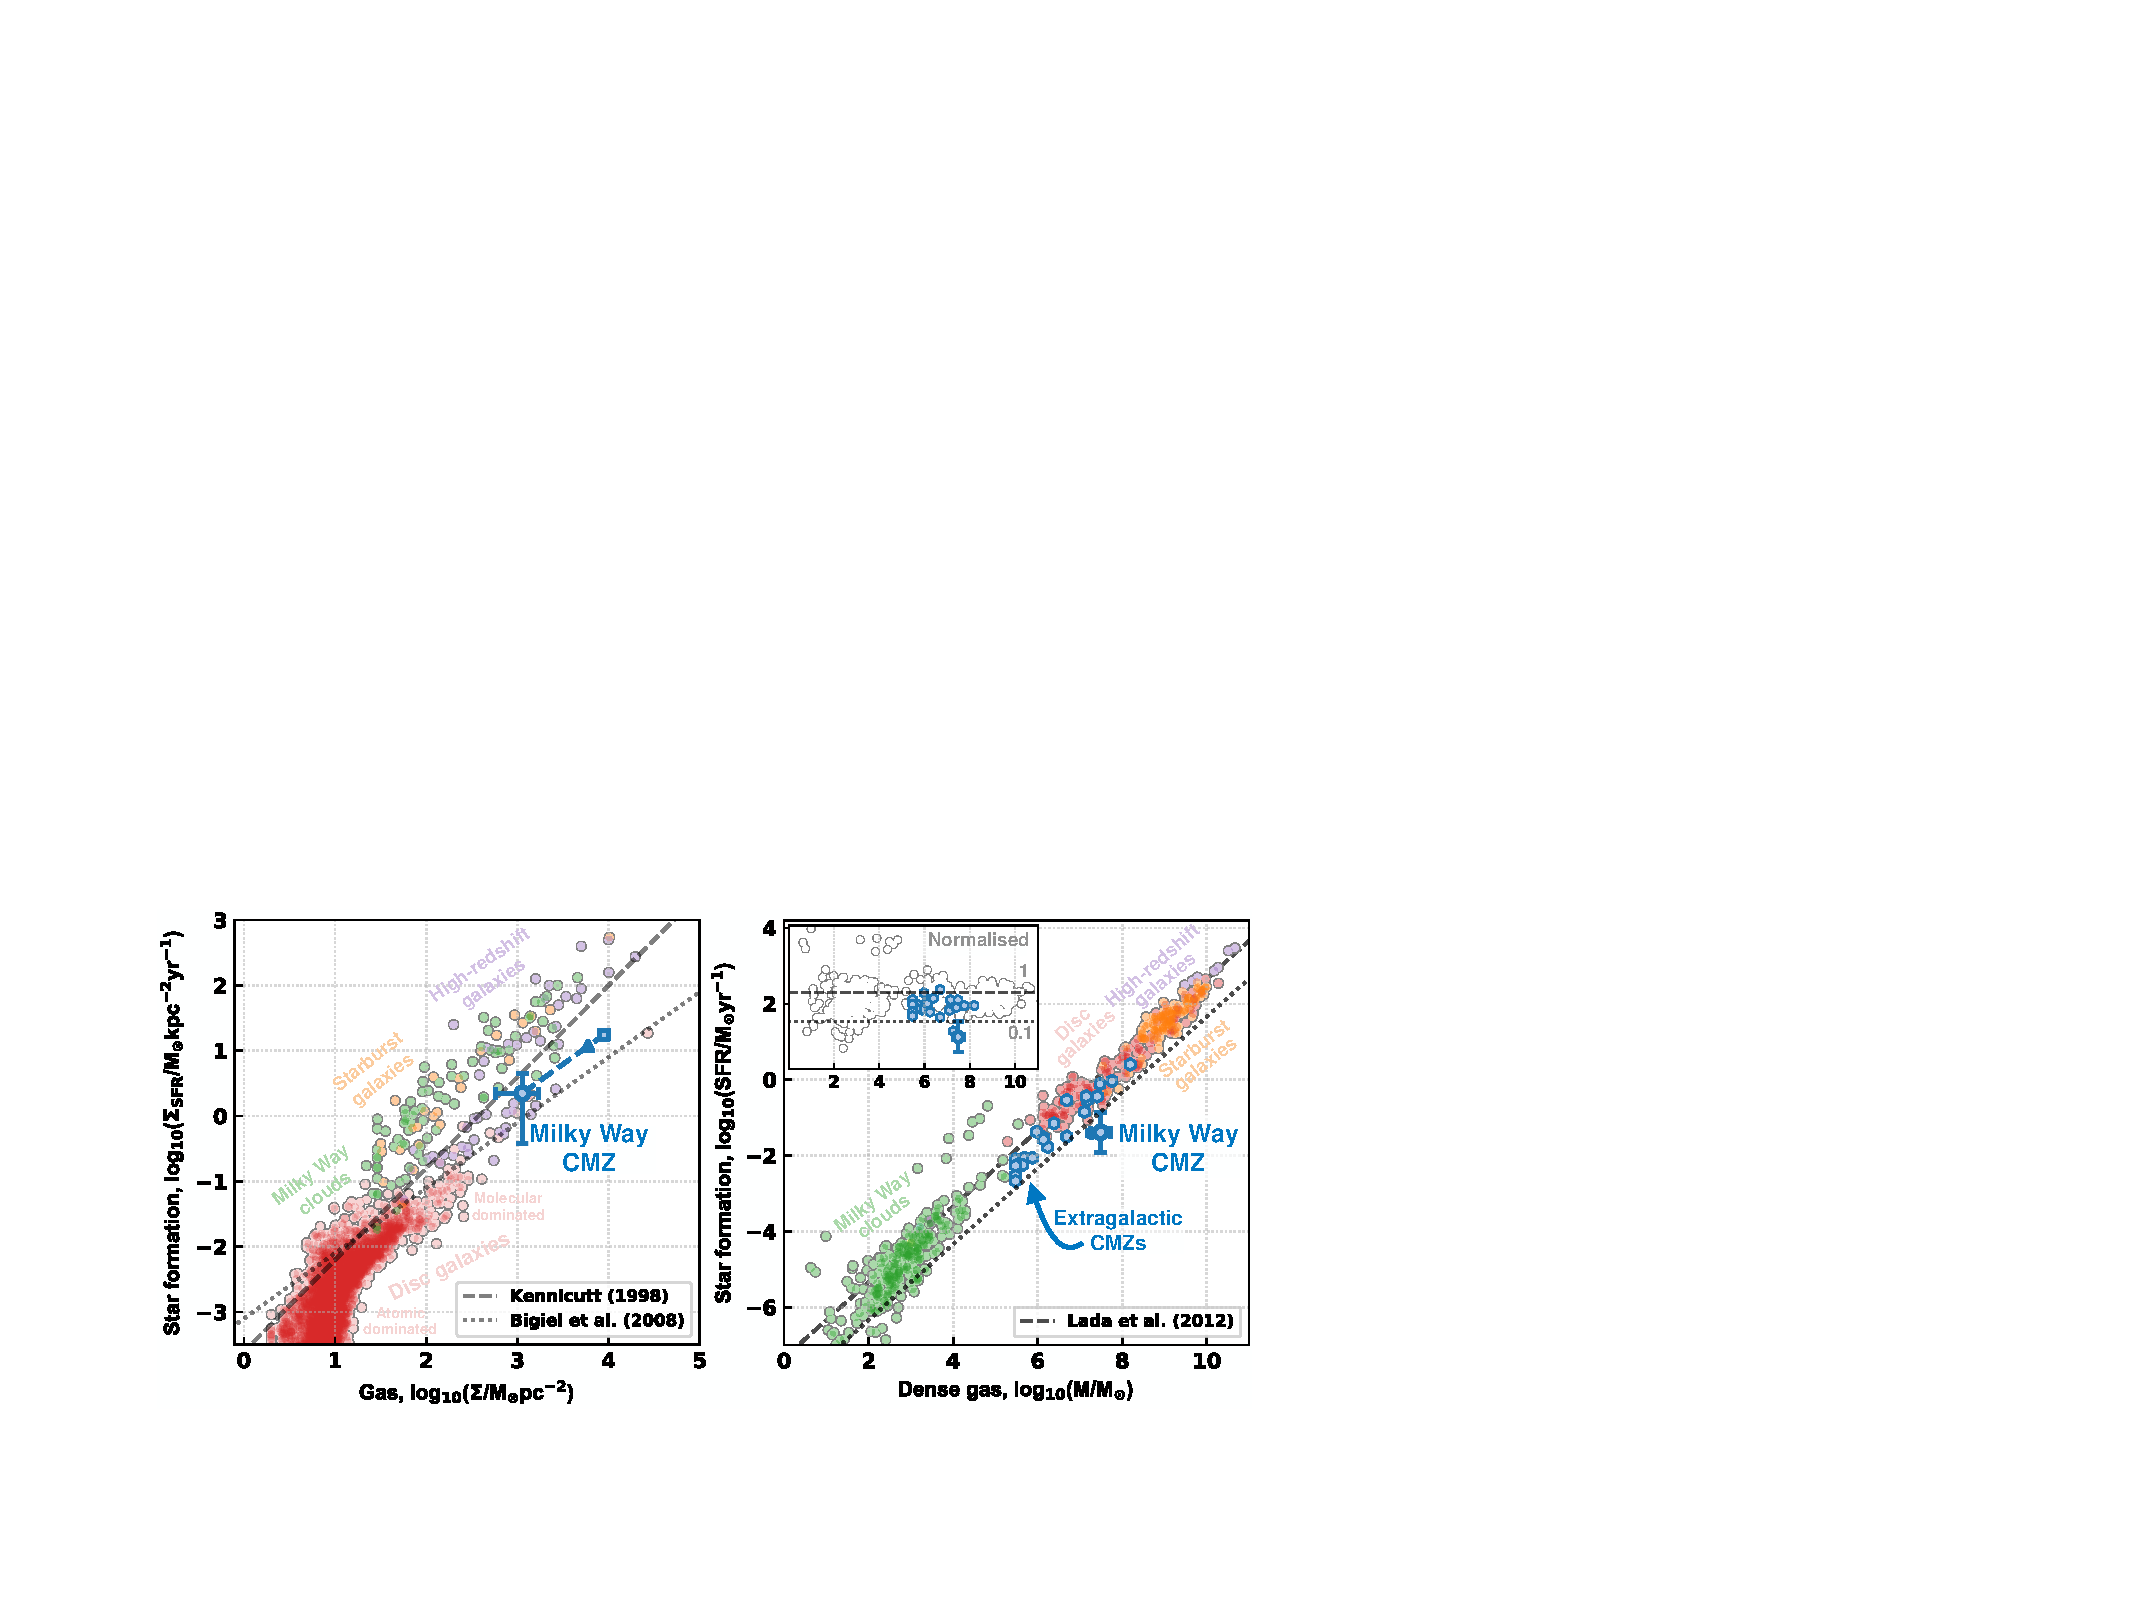
\includegraphics[trim=0 0cm 0 0cm, clip, width=0.85\textwidth]{./figs/sfr_compressed.pdf}
    \caption{The CMZ star-forming properties relative to several commonly used scaling relations. {\em Left:} The SFR surface density ($\Sigma_\mathrm{SFR}$) as a function of the gas surface density ($\Sigma_{\rm gas}$). The CMZ is shown by the large blue circle with error bars, which spans the range of $\Sigma_\mathrm{SFR}$ and $\Sigma_{\rm gas}$ determined in the literature (see Table\,\ref{tab:properties_overview}). This point is determined assuming a face-on disc geometry, whereas the connected points show the results of assuming either face-on ring (triangle) and edge-on geometry (square; see \S\,\ref{subsec:SFR:context}). Shown as grey-outlined coloured points are measurements of systems from the literature (see \citealp{Krumholz2014a} and references therein). Overplotted are the scaling relations from \citet{Kennicutt1998} and \citet{Bigiel2008}. {\em Right:} The relation between the dense molecular gas mass ($M_\mathrm{dense}$) and SFR. The CMZ is shown by the large blue circle with error bars, which span the range of $M_\mathrm{dense}$ and SFR determined in the literature (see Table\,\ref{tab:properties_overview}). Shown as grey-outlined coloured points are the values for systems taken from the literature (see \citealp{Jimenez-Donaire2019} for references). Shown as blue hexagons are extragalactic CMZs (\citealp{Querejeta2019,Jimenez-Donaire2019,Jiang2020,Beslic2021}). The dashed horizontal line shows the scaling relation of \citet{Lada2012}, and the dotted line shows a factor of ten below this relation. {\em Right (inset panel):} The $M_\mathrm{dense}$ and SFR/$M_\mathrm{dense}$, normalised to the \citet{Lada2012} relation.}
    \label{fig:sfr_main}
\end{figure*}


\begin{table*}[ht]
    \caption{Overview of bulk properties of the CMZ compared to the (order of magnitude) properties determined for the solar neighborhood, nearby extragalactic CMZs, and high-{\em z} Milky Way-like environments. 
    \label{tab:properties_overview}
    } \vspace{2mm}
    
    \centering
    \begin{tabular}{lcccc}
    \hline\hline
Physical Quantity                                  & CMZ                            & Solar Neighbourhood & Extragalactic CMZs & $z\sim2$  \\
\hline
Distance [kpc]$^{(a)}$                             & 8.2                            & 0.1 - 0.5           & 3500 - 20000       & $\sim$\,10$^6$ ({\em z}\,$\sim$\,2) \\
SFR [\msunyr]$^{(b)}$                              & 0.07 (0.012$\mhyphen$0.14)     & 0.002               & $0.001\mhyphen0.08$& 1-100\\
$\Sigma_{\rm gas}$ [log$_{10}$(\msunpc)]$^{(c)}$   & 3.1 (2.8$\mhyphen$3.2)         & 1.5                 & 0.6$\mhyphen$3     & 1.5$\mhyphen$3.5\\
$\Sigma_{\rm SFR}$ [log$_{10}$(\msunyrkpc)]$^{(d)}$& 0.3 ($-$0.4$\mhyphen$0.6)      & -2.5                & -3$\mhyphen$0      & -1.5$\mhyphen$1.5\\
$\Sigma_{*}$ [log$_{10}$(\msunpc)]$^{(e)}$         & 3.9                            & 1.5                 & 3.4$\mhyphen$3.9   & 1$\mhyphen$4 \\
$t_{\rm dep}$ [Gyr]$^{(f)}$             & 0.5 (0.4$\mhyphen$1.5)         & 1                   & $0.3\mhyphen2.6$          & 0.2$\mhyphen$1 \\
$t_{\rm dyn}$ [Myr]$^{(g)}$                        & 5                              & 220                 & 4-40               & ? \\
$B [\mu \mathrm{G}]$$^{(h)}$                       & 10$\mhyphen$1000               & 1$\mhyphen$100      & ?                  & ? \\
Metallicity, $Z$$^{(i)}$                           & 2                              & 1                   & $\sim$2            & 0.2$\mhyphen$0.6\\
CRIR [log$_{10}$(s$^{-1}$)]$^{(j)}$                & $-$15 to $-$13                 & $-$17 to $-$15      &  ?                 & ? \\
Linewidth, $\sigma(10 \mathrm{pc})$ [\kms]$^{(l)}$  & 12                            & 3                   & 10                 &  20$\mhyphen$70 \\
Linewidth scaling, $b$$^{(m)}$                      & 0.7                           & 0.5                 & ?                  &  ? \\
IMF slope, $\alpha$$^{(n)}$                         & $\leq$2.35                    & 2.35                & ?                  &  ? \\
DGMF, $f(n>10^4)$$^{(o)}$                           & 0.95                          & 0.03                & ?                  &  ? \\
$T_\mathrm{gas}$ [K]$^{(p)}$                        & 50$\mhyphen$100               & 10$\mhyphen$30      & 50$\mhyphen$250    & ? \\
$T_\mathrm{dust}$ [K]$^{(q)}$                       & 20$\mhyphen$50                & 10$\mhyphen$30      & 30$\mhyphen$45     & ? \\
$P_\mathrm{ext}/k_\mathrm{B}$ [K cm$^{-3}$]$^{(r)}$ & $\gtrsim10^7$                 & $\gtrsim10^5$       & $10^6\mhyphen10^8$  & ? \\ \hline
    \end{tabular}
    
    \begin{minipage}{\textwidth}\small
    \vspace{1mm} {\bf Notes:} References: $\{\mathrm{CMZ,\,Solar\ Neighbourhood,\,Extragalactic\ CMZ,\,}z\sim2\}$. The $\dagger$ symbol indicates values that are inferred from other properties in the table.
    $(a)$ Distance: $\{$\citet{GravityCollaboration2019}, --, --, -- $\}$.
    $(b)$ Star formation rate: $\{$\S~\ref{subsec:SFR:current}, \citet{Spilker2021}, \citet{Pessa2021}, \citet{Leslie2020}$\}$.
    $(c)$ Gas mass surface density: $\{$\S\ref{subsec:SFR:context}, \citet{Spilker2021}, Sun et al. (in prep.), \citet{Bolatto2015} $\}$.
    $(d)$ Star formation rate surface density: $\{$\S\ref{subsec:SFR:context}, \citet{Spilker2021}, \citet{Pessa2021}, \citet{Freundlich2013} $\}$.
    $(e)$ Stellar surface density: $\{$\citet{Sormani2021}, \citet{McKee2015}, \citet{Querejeta2015}, \citet{vanDokkum2010}$\}$. For the CMZ, we have considered the average value in a 100 pc radius circle.
    $(f)$ Depletion time, $\Sigma_{\rm gas}/\Sigma_{\rm SFR}$: $\{$$\dagger$, $\dagger$, Sun et al. (in prep.), \citet{Tacconi2020}$\}$.
    $(g)$ Dynamical or orbital time: $\{$\citet{Kruijssen2015}, \cite{Bland-Hawthorn2016}, \cite{Comeron2010}, -- $\}$.
    $(h)$ Magnetic field strength: $\{$\S~\ref{sec:magneticfields}, \citet{Chapman2011}, --, -- $\}$.
    $(i)$ Metallicity: $\{$\citet{Balser2011}, --, --, \citet{Maiolino2008} $\}$.
    $(j)$ Cosmic ray ionization rate: $\{$\S~\ref{sec:cosmicrays}, \citet{Neufeld2017}, --, -- $\}$.
    $(l)$ Linewidth: $\{$\citet{Shetty2012}, \citet{Heyer2015}, --, \citet{Swinbank2015} $\}$.
    $(m)$ Size-Linewidth relationship scaling: $\{$\S~\ref{sec:velocitystructure}, \citet{Heyer2015}, --, -- $\}$.
    $(n)$ Stellar initial mass function slope: $\{$\S~\ref{sec:starclusters}, \citet{Offner2014}, --, -- $\}$.
    $(o)$ Dense gas fraction, or fraction of mass above $n>10^{3\mhyphen4}$\,\cmc: $\{$\citet{Longmore2013b}, \citet{Spilker2021}, --, -- $\}$.
    $(p)$ Molecular gas temperature: $\{$\citet{Krieger2017}, \citet{Friesen2017}, \citet{Mangum2013}, -- $\}$.
    $(q)$ Dust temperature: $\{$\citet{Tang2021a}, \citet{Chen2016}, \citet{Mangum2013}, -- $\}$.
    $(r)$ External pressure: $\{$\citet{Myers2022}, \citet{Field2011}, \citet{Sun2020b}, -- $\}$
    \end{minipage}
    
\end{table*}

A key development that emerged around the time of Protostars \& Planets VI was that the current SFR of \linebreak $\simeq0.07$\,\msunyr \ (\S\ref{subsec:SFR:current} and \S\ref{subsec:SFR:past}; Table\,\ref{tab:SFR}) is an order of magnitude below that expected for the available reservoir of dense molecular gas in the CMZ \citep{Longmore2013b}.
This expectation comes from so-called star formation scaling relations, which are empirical correlations describing the relationship between the rate at which stars form and the properties of the ISM out of which they are born.

Perhaps the most familiar of these scaling relations is the ``Schmidt–Kennicutt'' relation \citep[][hereafter SK relation]{Schmidt1959,Kennicutt1998}, which describes the correlation between the SFR surface density, $\Sigma_\mathrm{SFR}$, and the total gas surface density, $\Sigma_{\rm gas}$ ($\Sigma_\mathrm{SFR}\propto\Sigma_{\rm gas}^{n}$, where $n=1.4$; see the dashed line in the left panel of Fig.~\ref{fig:sfr_main}). Because of the non-linearity of the SK relation, the degree to which the CMZ agrees (or disagrees) with it depends on geometrical assumptions. \citet{Yusef-Zadeh2009} argued that the central 400\,pc of the Galaxy appears to be forming stars in accordance with the SK relation if the gas surface density is calculated using the area projected on the sky and using their measured value of the SFR (which was probably overestimated, see \S \ref{subsec:SFR:current}). \citet{Kruijssen2014a} instead calculated the surface densities assuming that the gas and star formation in the CMZ are distributed throughout a 100-pc ring/annulus with a width of 10\,pc, i.e. $\Sigma_{\rm gas}=M_\mathrm{gas}\pi^{-1}(R_1^2-R_2^2)^{-1}$, where $R_1-R_2$ is the width of the annulus \citep[see also][]{Longmore2013b}. Under this assumption, they found that the 100-pc ring is forming stars at a rate that is $\sim$ an order of magnitude below the SK relation. We illustrate the effect of different geometrical assumptions for the CMZ (a 100\,pc ring/annulus, a 100\,pc disc, and the projected area on the sky) in the left panel of Fig.~\ref{fig:sfr_main}. 
In conclusion, depending on the assumed geometry, the CMZ appears to be roughly consistent, or at most marginally inconsistent, with the SK relation, taking into account the considerable typical scatter around this relation.

\citet{Kruijssen2014a} showed that the CMZ is consistent with the \citet{Bigiel2008} relation, which describes the linear relationship between the molecular (as opposed to total) gas surface density and the SFR ($\Sigma_\mathrm{SFR}\propto\Sigma_\mathrm{mol}$; see the dotted line in the left panel of Fig.~\ref{fig:sfr_main}).
They commented that this agreement is surprising, since dynamical evolution should proceed faster under the influence of self-gravity when the surface density is higher (i.e. $n>1$). The long depletion time implied by the \cite{Bigiel2008} relation ($t_\mathrm{dep}\sim1\mhyphen2$\,Gyr) perhaps indicates that some mechanism is inhibiting star formation in the CMZ (also see e.g. \citealp{Sofue2017b} and \citealp{Sofue2017c} for varying $\Sigma_\mathrm{SFR}\mhyphen\Sigma$ relations within the Galaxy). 

A star formation relation that the CMZ is clearly inconsistent with is the so-called dense gas star formation relation (e.g. see \citealp{Longmore2013b}), which is a linear relation between the total SFR and the mass of dense molecular gas (i.e.\ gas denser than that traced by CO), $M_\mathrm{dg}$. This relation was first proposed by \citet{Gao2004}, using global measurements of external galaxies in which the amount of dense gas was inferred from the luminosity of HCN. \citet{Lada2010,Lada2012} extended this relationship to Milky Way clouds, and found that SFR is directly proportional to the mass of gas above a constant surface density threshold of $\Sigma_\mathrm{gas} \approx 116$\,\msun~pc$^{-2}$. This tight correlation appears to hold well both for nearby molecular clouds and for external galaxies (see the dashed line in the right panel of Fig.~\ref{fig:sfr_main}). 

The vast majority of the gas in the CMZ is above the density threshold proposed by 
\citet{Lada2010,Lada2012}. \citet{Longmore2013b} showed that the CMZ is presently under-producing stars by an order of magnitude relative to the SFR that would be predicted by the dense gas scaling relation (see inset panel in Fig.~\ref{fig:sfr_main}).
This is a strong counterargument against the notion of a constant surface density threshold for star formation. 
Clearly, star formation in the CMZ does not only depend on the amount of available dense gas, and other environmental factors are probably important \citep[][we will return to this topic in the context of individual clouds in \S\ref{sec:sfthreshold}]{Longmore2013b, Kruijssen2014a, Rathborne2014a, Ginsburg2018a}.

Observations of extragalactic nuclei may help to provide some further insight. 
Studies of the central $\sim$\,1\,kpc regions of external galaxies have found higher dense gas fractions and lower dense gas star formation efficiencies ($\mathrm{SFR}/M_\mathrm{dense}$), similar to the CMZ (see e.g.\ \citealp{Usero2015,Bigiel2016,Jimenez-Donaire2019,Querejeta2019,Beslic2021,Eibensteiner2022}). 
However, the current sample of resolved observations of extragalactic CMZs is very small. Further resolved observations of nearby galactic nuclei are needed to better understand whether the CMZ represents an outlier, or if other CMZs are similarly inconsistent with the dense gas star formation relation.

\subsection{Star formation history}
\label{subsec:SFR:starformationhistory}

The star formation history (SFH) of the CMZ is encoded within the stellar populations of the Nuclear Bulge (NB, $R<300\pc$) and in particular of the Nuclear Stellar Disc (NSD; \citealt{Launhardt2002}). 
For a long time it was believed that the NSD has been built up by quasi-continuous star formation occurring over the last $\sim 10\, \gyr$ \citep{Figer2004}. 
A quasi-continuous SFR may seem natural. 
After all, the different methods outlined in \S\ref{sec:SFR:current} suggest that the ``present-day'' SFR is comparable to that averaged over the past $5\mhyphen100$\,Myr within a factor of two \citep{Barnes2017}. 
And if we assume that the SFR has remained roughly constant at the present value of $0.07$ \msunyr \ over this $\sim 10\, \gyr$ time frame, we obtain a total mass of $7 \times 10^8$ \msun, which is strikingly similar to the current mass of the NSD \citep{Sormani2021}.
Furthermore, \citet{Matsunaga2011}, based on the presence of classical cepheids with ages well-determined from their pulsation periods, found that the SFR in the CMZ between 20-30 \myr \ ago was $0.075^{+0.15}_{-0.05}$\,\msunyr \ , very close to the present value.

However, \cite{Nogueras-Lara2020b} recently challenged the view of a quasi-continuous SFR using data from the GALACTICNUCLEUS survey. 
They modelled the extinction-corrected K-band colour-magnitude diagram over extended regions of the NSD as a superposition of star formation events occurring at different times. 
They concluded that $\sim 80 \%$ of the stars in the NSD formed more than $8\, \gyr$ ago, followed by a drop in star formation activity between $8\,\gyr$ and $1\, \gyr$ ago. 
They also found that the SFR has been variable during the past $1\, \gyr$, with periods of more intense activity (SFR$\sim 0.5\, \msun \peryr$). They found a SFR of $\sim0.1$ \msunyr \ averaged over the past 100 \myr, in accordance with the estimates in \S\ref{subsec:SFR:past}, and of $0.2\mhyphen0.8\, \msun \peryr$ in the past 30 \myr, i.e.\ a factor of a few higher than the present-day value (\S\ref{subsec:SFR:current}).

The CMZ also contains two young massive clusters known as the Arches and Quintuplet, which both formed $\lesssim5$\,Myr ago (\S\ref{sec:starclusters}), and the central parsec contains of the order 200 young ($\sim3\mhyphen6$\,Myr) high-mass stars \citep{Genzel2010, Lu2013}. In the context of present-day star formation, some work \citep[e.g.][]{Lu2019b} suggests the possibility that the SFR is currently increasing (\S\ref{sec:sfinaction}), though this is not strongly evidenced in full CMZ studies \citep{Hatchfield2020, Battersby2020}. Taken together, this evidence could suggest that the CMZ has experienced short bursts of star formation activity which are averaged out in integrated light measurements (\S\ref{subsec:SFR:past}).

Though the sample size is small, there is some evidence suggesting that star formation in extragalactic nuclei may also proceed episodically in discrete bursts. \cite{Allard2006} analysed the SFH in the nuclear ring of the barred galaxy NGC 4321 and found that star formation in the last $500\, \myr$ proceeded in a succession of bursts separated by roughly $\sim 100\, \myr$. \cite{Sarzi2007} extended this analysis to a sample of 8 nearby galaxies and found similar results, concluding that star formation is more likely to proceed in episodic bursts rather than continuously. \cite{Prieto2019} derived ages for 171 star clusters in the nuclear ring of NGC 1097 
by fitting SEDs in the UV and IR range, and concluded that the ring has been subject to intermittent bursts of star formation spread over the last few $100\, \myr$ with a time separation of about $20$-$30\,\myr$ (finer time separations are not resolved). \cite{Callanan2021} combined ALMA observations with ages of massive clusters derived from \citet{Harris2001} to argue that the nuclear ring in M83 experienced a starburst $5\mhyphen7\, \myr$ ago which was highly localised in time. On longer timescales, \cite{Gadotti2019} derived the SFHs in the nuclear regions of two selected galaxies in the sample of the TIMER survey, NGC 1097 and NGC 4643, with a temporal resolution of $\sim 700 \, \myr$, and found that NGC 1097 exhibits two starbursts episodes $\sim 0.5$\,Gyr and $\sim 2.5$\,Gyr ago respectively (in addition to the one that is ongoing now), while NGC 4643 does not show signs of burst activity at the temporal resolution allowed by the data. 

In conclusion, there is now clear evidence that the SFR in the CMZ has varied significantly over the past few tens to hundreds of Myrs, and that the SFRs of galactic nuclei, in general, vary considerably as a function of time.

\subsection{What drives the time evolution of star formation in galactic nuclei?}
\label{subsec:SFR:timeevolution}

Although there is evidence to suggest that star formation in the CMZ has varied significantly in the past, and that bursts of star formation activity may occur in galactic nuclei more generally, it is currently debated what may drive such variations in the SFR. 
If star formation in the CMZ is episodic, this could explain the present discrepancy between the CMZ and some of the star formation relations discussed in \S\ref{subsec:SFR:context}. 
In this context, the \emph{time-averaged} SFR of the CMZ may be consistent with star formation scaling relations, even if the CMZ is currently at a low point in its star formation history \citep{Kruijssen2014a, Krumholz2015}. 

One way to explain the variable SFR, based on semi-analytical or simple 1D hydrodynamical models, is that stellar feedback drives a recurrent cycle of star formation \citep{Loose1982,Krugel1993,Elmegreen1994,Morris1996,Stark2004,Kruijssen2014a,Krumholz2015,Krumholz2017,Torrey2017}. The common idea of all these models is that gas accumulates in the central region until a starburst occurs. This starburst releases a great amount of energy that temporarily halts star formation, and once that turbulent energy dissipates, the cycle repeats. The predicted time intervals between the bursts range between $\sim 20$\,Myr \citep{Krumholz2017} to $\sim 100$\,Myr \citep{Loose1982}. 

Various authors have recently tested this picture using full 3D simulations, finding contrasting results. \cite{Torrey2017} ran numerical simulations of isolated galaxies with the FIRE feedback model and found that the SFR within the central $\sim100$\,pc goes through dramatic, oscillatory cycles. \cite{Armillotta2019} performed simulations of the Milky Way in the rigidly-rotating barred gravitational potential of \cite{Ridley2017}. They found that the CMZ SFR varies by $\approx1.5$ dex over a timespan of $\sim 500\,\myr$, even though the gas mass in the CMZ stays relatively constant (implying large variations in the depletion time). This variability occurs in cycles of $50\,\myr$ and is driven by stellar feedback, in accordance with the expectations of the 1D models. 

However, \cite{Sormani2020b}, using a similar setup to that of \citet{Armillotta2019}, found that stellar feedback does not drive cycles of star formation in their simulations. Rather, they found that the SFR is quite steady and directly proportional to the time-varying CMZ mass (implying a roughly constant depletion time). \cite{Moon2021} performed semi-global hydrodynamic simulations of nuclear rings subject to constant mass inflow rates (to avoid the time-variability that naturally arises in fully global simulations) and found that the SFR exhibits only modest (within a factor of $\sim$2) temporal fluctuations, similar to \cite{Sormani2020b}. 
Finally, \citet{Orr2021} perform cosmological zoom simulations of seven Milky Way mass galaxies from FIRE-2 and find a mix of the two pictures described above. They identify two classes of galaxy centres: one with highly asymmetric gas and SFR distributions, which undergo rapid SFR variations on 10 Myr timescales, and another with smooth gas and SFR distributions. 

The origin of the diverse results obtained from the simulations mentioned above is not clear. The absence of the boom/bust behaviour in the simulations of \cite{Sormani2020b} and \cite{Moon2021} may be because they only include supernova feedback but lack early feedback such as stellar winds, photoionization, and radiation pressure from young stars \citep[which can disperse gas to parsec scales surrounding sites of star formation before the onset of the first supernova;][]{Barnes2020b}. Alternatively, the simulations of \cite{Armillotta2019} may not be sufficiently resolved and thus produce numerical artefacts \citep{Sormani2020b,Moon2021}. Addressing the origin of the contrasting simulation results described above will require careful comparison of the different ways of implementing star formation and feedback in the simulations.

Alternatively (or in addition) to stellar feedback cycles, variations in the SFR may also reflect time variability in the mass inflow rate \citep[][]{Seo2019,Sormani2020b, Moon2022}. Observations of the Milky Way \citep{Sormani2019b} and external galaxies \citep{Leroy2021, Beslic2021} often show that the dust lanes, which transport the gas to the centre, contain dense clumps that may produce discrete large accretion events. 
\citet{Moon2022} used simulations to study SFR variability resulting from a controlled oscillating inflow rate. 
They found that if the inflow oscillations have sufficient amplitude they can cause large (a factor of $>5$) fluctuations of the SFR over timescales of $\Delta t > 50$ Myr. Finally, starbursts may be also produced by perturbations induced by a live stellar potential \citep[][as opposed to the fixed potential in the above simulations]{Emsellem2015} or minor mergers \citep{Mihos1994}, while AGN activity might quench star formation by blowing the gas out \citep{Combes2017a}.

In conclusion, the main driver of SFR variations in the CMZ is currently unclear, though the main candidates are stellar-feedback-driven star formation cycles and a variable bar-driven inflow rate. There are good prospects that numerical simulations will soon be able to determine whether the former is a physically viable mechanism, while insight on the latter might come from studying nearby barred galaxies.